\documentclass{article}

\usepackage{geometry}
\usepackage{amsmath}
\usepackage{graphicx, eso-pic}
\usepackage{listings}
\usepackage{hyperref}
\usepackage{multicol}
\usepackage{fancyhdr}
\pagestyle{fancy}
\fancyhf{}
\hypersetup{ colorlinks=true, linkcolor=black, filecolor=magenta, urlcolor=cyan}
\geometry{ a4paper, total={170mm,257mm}, top=40mm, right=20mm, bottom=20mm, left=20mm}
\setlength{\parindent}{0pt}
\setlength{\parskip}{0.5em}
\renewcommand{\headrulewidth}{0pt}
\AddToShipoutPictureBG{%
  \AtPageUpperLeft{%
    \raisebox{-\height}{
\includegraphics[width=\paperwidth, height=30mm]{../headerarkav.png}}
  }
}
\rfoot{\thepage}
\lfoot{Competitive Programming - Arkavidia 8.0}
\lstset{
    basicstyle=\ttfamily\small,
    columns=fixed,
    extendedchars=true,
    breaklines=true,
    tabsize=2,
    prebreak=\raisebox{0ex}[0ex][0ex]{\ensuremath{\hookleftarrow}},
    frame=none,
    showtabs=false,
    showspaces=false,
    showstringspaces=false,
    prebreak={},
    keywordstyle=\color[rgb]{0.627,0.126,0.941},
    commentstyle=\color[rgb]{0.133,0.545,0.133},
    stringstyle=\color[rgb]{01,0,0},
    captionpos=t,
    escapeinside={(\%}{\%)}
}

\begin{document}

\begin{center}
    \section*{H. Hexagame} % ganti judul soal

    \begin{tabular}{ | c c | }
        \hline
        Batas Waktu  & 2s \\    % jangan lupa ganti time limit
        Batas Memori & 128MB \\  % jangan lupa ganti memory limit
        \hline
    \end{tabular}
\end{center}

\subsection*{Deskripsi}
Arka dan Vidia sedang bermain game melawan satu sama lain pada papan petak heksagonal tak hingga. Game ini disebut dengan \textbf{Hexagame}. Setiap petak pada papan heksagonal memiliki koordinat sepasang bilangan bulat yang berkorespondensi pada 2 sumbu seperti gambar ini. 

\begin{center}
    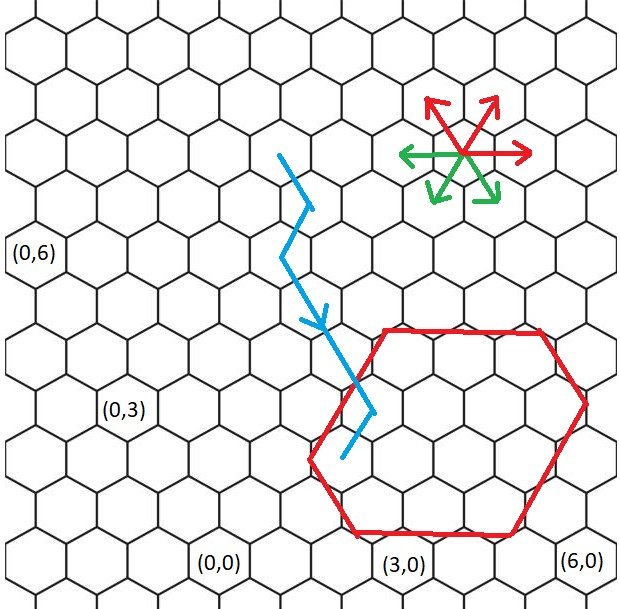
\includegraphics[scale = 0.4]{hexagon.jpg}
\end{center}

Permainan \textbf{Hexagame} diawali dengan sebuah batu yang berada pada koordinat ($X_0$,$Y_0$) dan sebuah bilangan $K$ dengan $X_0$, $Y_0$, dan $K$ bilangan asli. Pada setiap langkah, pemain dapat melakukan pergeseran ke salah satu dari 3 arah (kiri, bawah-kiri, dan bawah-kanan) minimal 1 kali dan maksimal K kali. Sebuah \textbf{pergeseran} didefinisikan sebagai pergerakan sebuah benda dari suatu petak ke salah satu dari 6 petak yang persis menyentuhnya. Pada gambar diatas, 3 arah pergeseran yang dapat dilakukan oleh pemain ditandai panah berwarna hijau. Pada permainan ini, terdapat aturan sebagai berikut.

\begin{enumerate}
  \item Pemain tidak dapat menggeser batu ke petak dengan salah satu koordinat bernilai negatif.
  \item Arka selalu mendapat giliran pertama.
  \item Pemain yang dapat menggeser batu ke (0,0) dinyatakan sebagai pemenangnya.
\end{enumerate}

Didefinisikan sebuah petak dengan koordinat ($X$,$Y$) sebagai petak \textbf{GG} apabila Arka memiliki strategi pasti untuk menang pada permainan yang dimulai dari koordinat awal $(X_0, Y_0) = (X,Y)$. Didefinisikan pula sebuah \textbf{Area} seperti pada gambar, merupakan daerah hexagonal konveks yang didefinisikan dari tepat 3 titik sudutnya $(A,B),(C,D),(E,F)$ yang memenuhi aturan sebagai berikut.
\begin{enumerate}
  \item $A \leq C \leq E$
  \item $D \leq B \leq F$
  \item $A-B \leq E-F \leq C-D$
  \item $F-B \leq C-A$
\end{enumerate} 

Pada contoh, terdapat 14 petak dalam daerah yang memiliki sudut (3,2),(5,1),(7,4). Carilah jumlah petak GG dari gabungan (union) $N$ area berbeda.

\subsection*{Format Masukan}
Baris pertama berisi $N$ dan $K$ ( $1 \leq N \leq 1000$, $1 \leq K \leq 10^6$).

$N$ baris berikutnya berisi 6 bilangan $A_i, B_i, C_i, D_i, E_i, F_i$ yang menyatakan area ke-i dengan ($0 \leq A_i, B_i, C_i, D_i, E_i, F_i < 10^9$).

\subsection*{Format Keluaran}
Keluarkan satu angka yang menyatakan banyak petak GG yang termasuk dalam paling tidak satu area yang dimodulo $10^9+7$.

\begin{multicols}{2}
\subsection*{Contoh Masukan}
\begin{lstlisting}
  3 1
  0 6 1 3 3 7
  5 8 7 4 9 8
  1 3 4 2 7 6
\end{lstlisting}
\columnbreak

\subsection*{Contoh Keluaran}
\begin{lstlisting}
37
\end{lstlisting}
\vfill
\null
\end{multicols}

\subsection*{Penjelasan}
Pada contoh masukan di atas, terdapat 3 area yang didefinisikan oleh 3 pasang titik sudut. Area pertama memiliki titik sudut (0,6),(1,3),(3,7). Area kedua memiliki titik sudut (5,8),(7,4),(9,8). Area ketiga memiliki titik sudut (1,3),(4,2),(7,6). Berikut adalah gambaran dari 3 area tersebut.

\begin{center}
    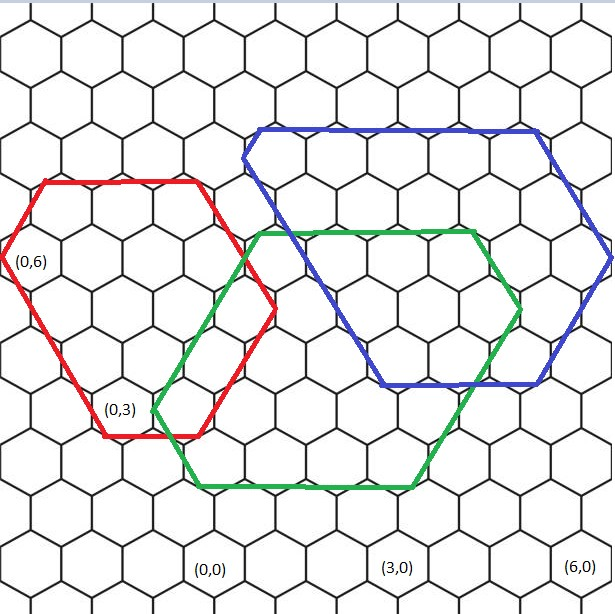
\includegraphics[scale = 0.4]{hexagon2.jpg}
\end{center}

Dari gambar di atas, terdapat 41 petak GG yang termasuk dalam paling tidak satu area dengan rincian sebagai berikut.
\begin{enumerate}
  \item Pada area pertama (ditandai warna merah), terdapat 16 petak, 12 diantaranya GG.
  \item Pada area kedua (ditandai warna biru), terdapat 22 petak, 17 diantaranya GG.
  \item Pada area ketiga (ditandai warna hijau), terdapat 23 petak, 16 diantaranya GG.
  \item Pada irisan area pertama dan ketiga, terdapat 3 petak, 2 diantaranya GG.
  \item Pada irisan area kedua dan ketiga, terdapat 8 petak, 6 diantaranya GG.
  \item Tidak ada irisan area pertama dan kedua
  \item Tidak ada irisan pada ketiga area sekaligus
\end{enumerate}

Oleh karena itu, gabungan ketiga area terdapat 50 petak, 37 diantaranya GG

\end{document}